\documentclass[tikz]{standalone}
\usepackage{amsmath}
\definecolor{bg}{HTML}{171D2B}
\definecolor{aksen}{HTML}{F7B538}
\begin{document}
\pagecolor{bg}
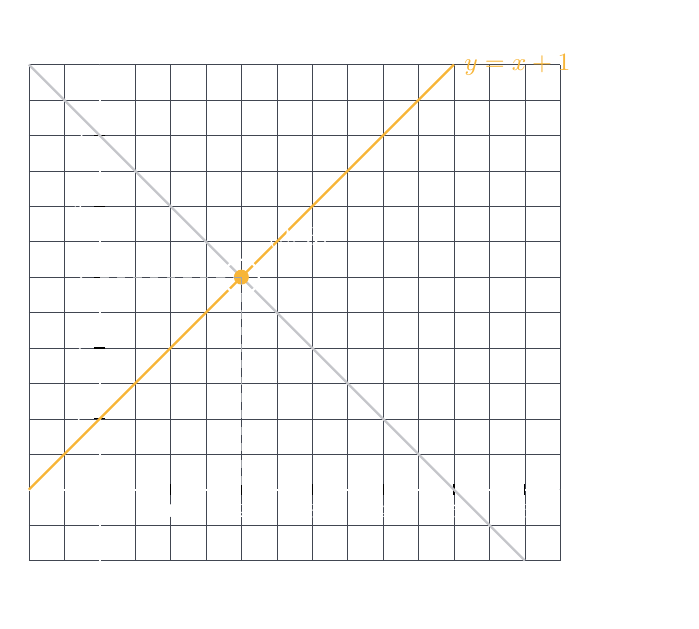
\begin{tikzpicture}[scale=0.9,>=stealth,
  garis1/.style={thick,aksen},
  garis2/.style={thick,white!75!bg},
  gridline/.style={very thin,white!18!bg}]
  % grid
  \foreach \x in {-1,-0.5,...,6.5} \draw[gridline] (\x,-1) -- (\x,6);
  \foreach \y in {-1,-0.5,...,6} \draw[gridline] (-1,\y) -- (6.5,\y);
  % axes
  \draw[->,thick,white] (-1,0) -- (6.5,0) node[right]{\color{white}$x$};
  \draw[->,thick,white] (0,-1) -- (0,6) node[above]{\color{white}$y$};
  \foreach \x in {1,...,6} \draw (\x,0.08) -- (\x,-0.08) node[below]{\color{white}\scriptsize $\x$};
  \foreach \y in {1,...,5} \draw (0.08,\y) -- (-0.08,\y) node[left]{\color{white}\scriptsize $\y$};
  % garis 1: y = x + 1
  \draw[garis1] (-1,0) -- (5,6) node[right,aksen]{\color{aksen}\small $y=x+1$};
  % garis 2: y = -x + 5
  \draw[garis2] (-1,6) -- (6,-1) node[below right,white]{\color{white}\small $y=-x+5$};
  % titik potong (2,3)
  \fill[aksen] (2,3) circle (3pt);
  \draw[white,thick] (2,3) circle (7pt);
  \node[above right=6pt] at (2,3) {\color{white}\small $(2,\,3)$};
  % garis bantu
  \draw[dashed,white!60!bg] (2,3) -- (2,0);
  \draw[dashed,white!60!bg] (2,3) -- (0,3);
\end{tikzpicture}
\end{document}
